% Figure s02f03_blochrecipe (Session 2): band folding, the two-band chain seen from the one-band chain.
% The image is rendered by figures/blender/s02f03_blochrecipe.py; the coordinates of the labels come from
% figures/blender/out/s02f03_blochrecipe_anchors.tex. Build with figures/blender/build_figure.sh s02f03_blochrecipe.
\documentclass[11pt,tikz,border=0pt]{standalone}
\usepackage[T1]{fontenc}
\usepackage{amsmath,amssymb,graphicx,bm}
\usepackage{xcolor}
\usetikzlibrary{arrows.meta,calc}
% The three label colors of the figures, with the same values as in src/figures_preamble.tex.
\definecolor{aqmaccent}{RGB}{31,78,121}
\definecolor{aqmbroken}{RGB}{168,42,34}
\definecolor{aqmmuted}{RGB}{125,125,125}

\newlength{\figw}\setlength{\figw}{15.6cm}   % the text width of the notes (A4, 2.7 cm margins)

\begin{document}
\begin{tikzpicture}[lbl/.style={font=\small, inner sep=1.5pt}, pnl/.style={font=\small\bfseries, inner sep=1.5pt}]
  \begin{scope}
    \setlength{\figw}{4.4cm}
    \node[anchor=south west, inner sep=0pt] at (0,0)
      {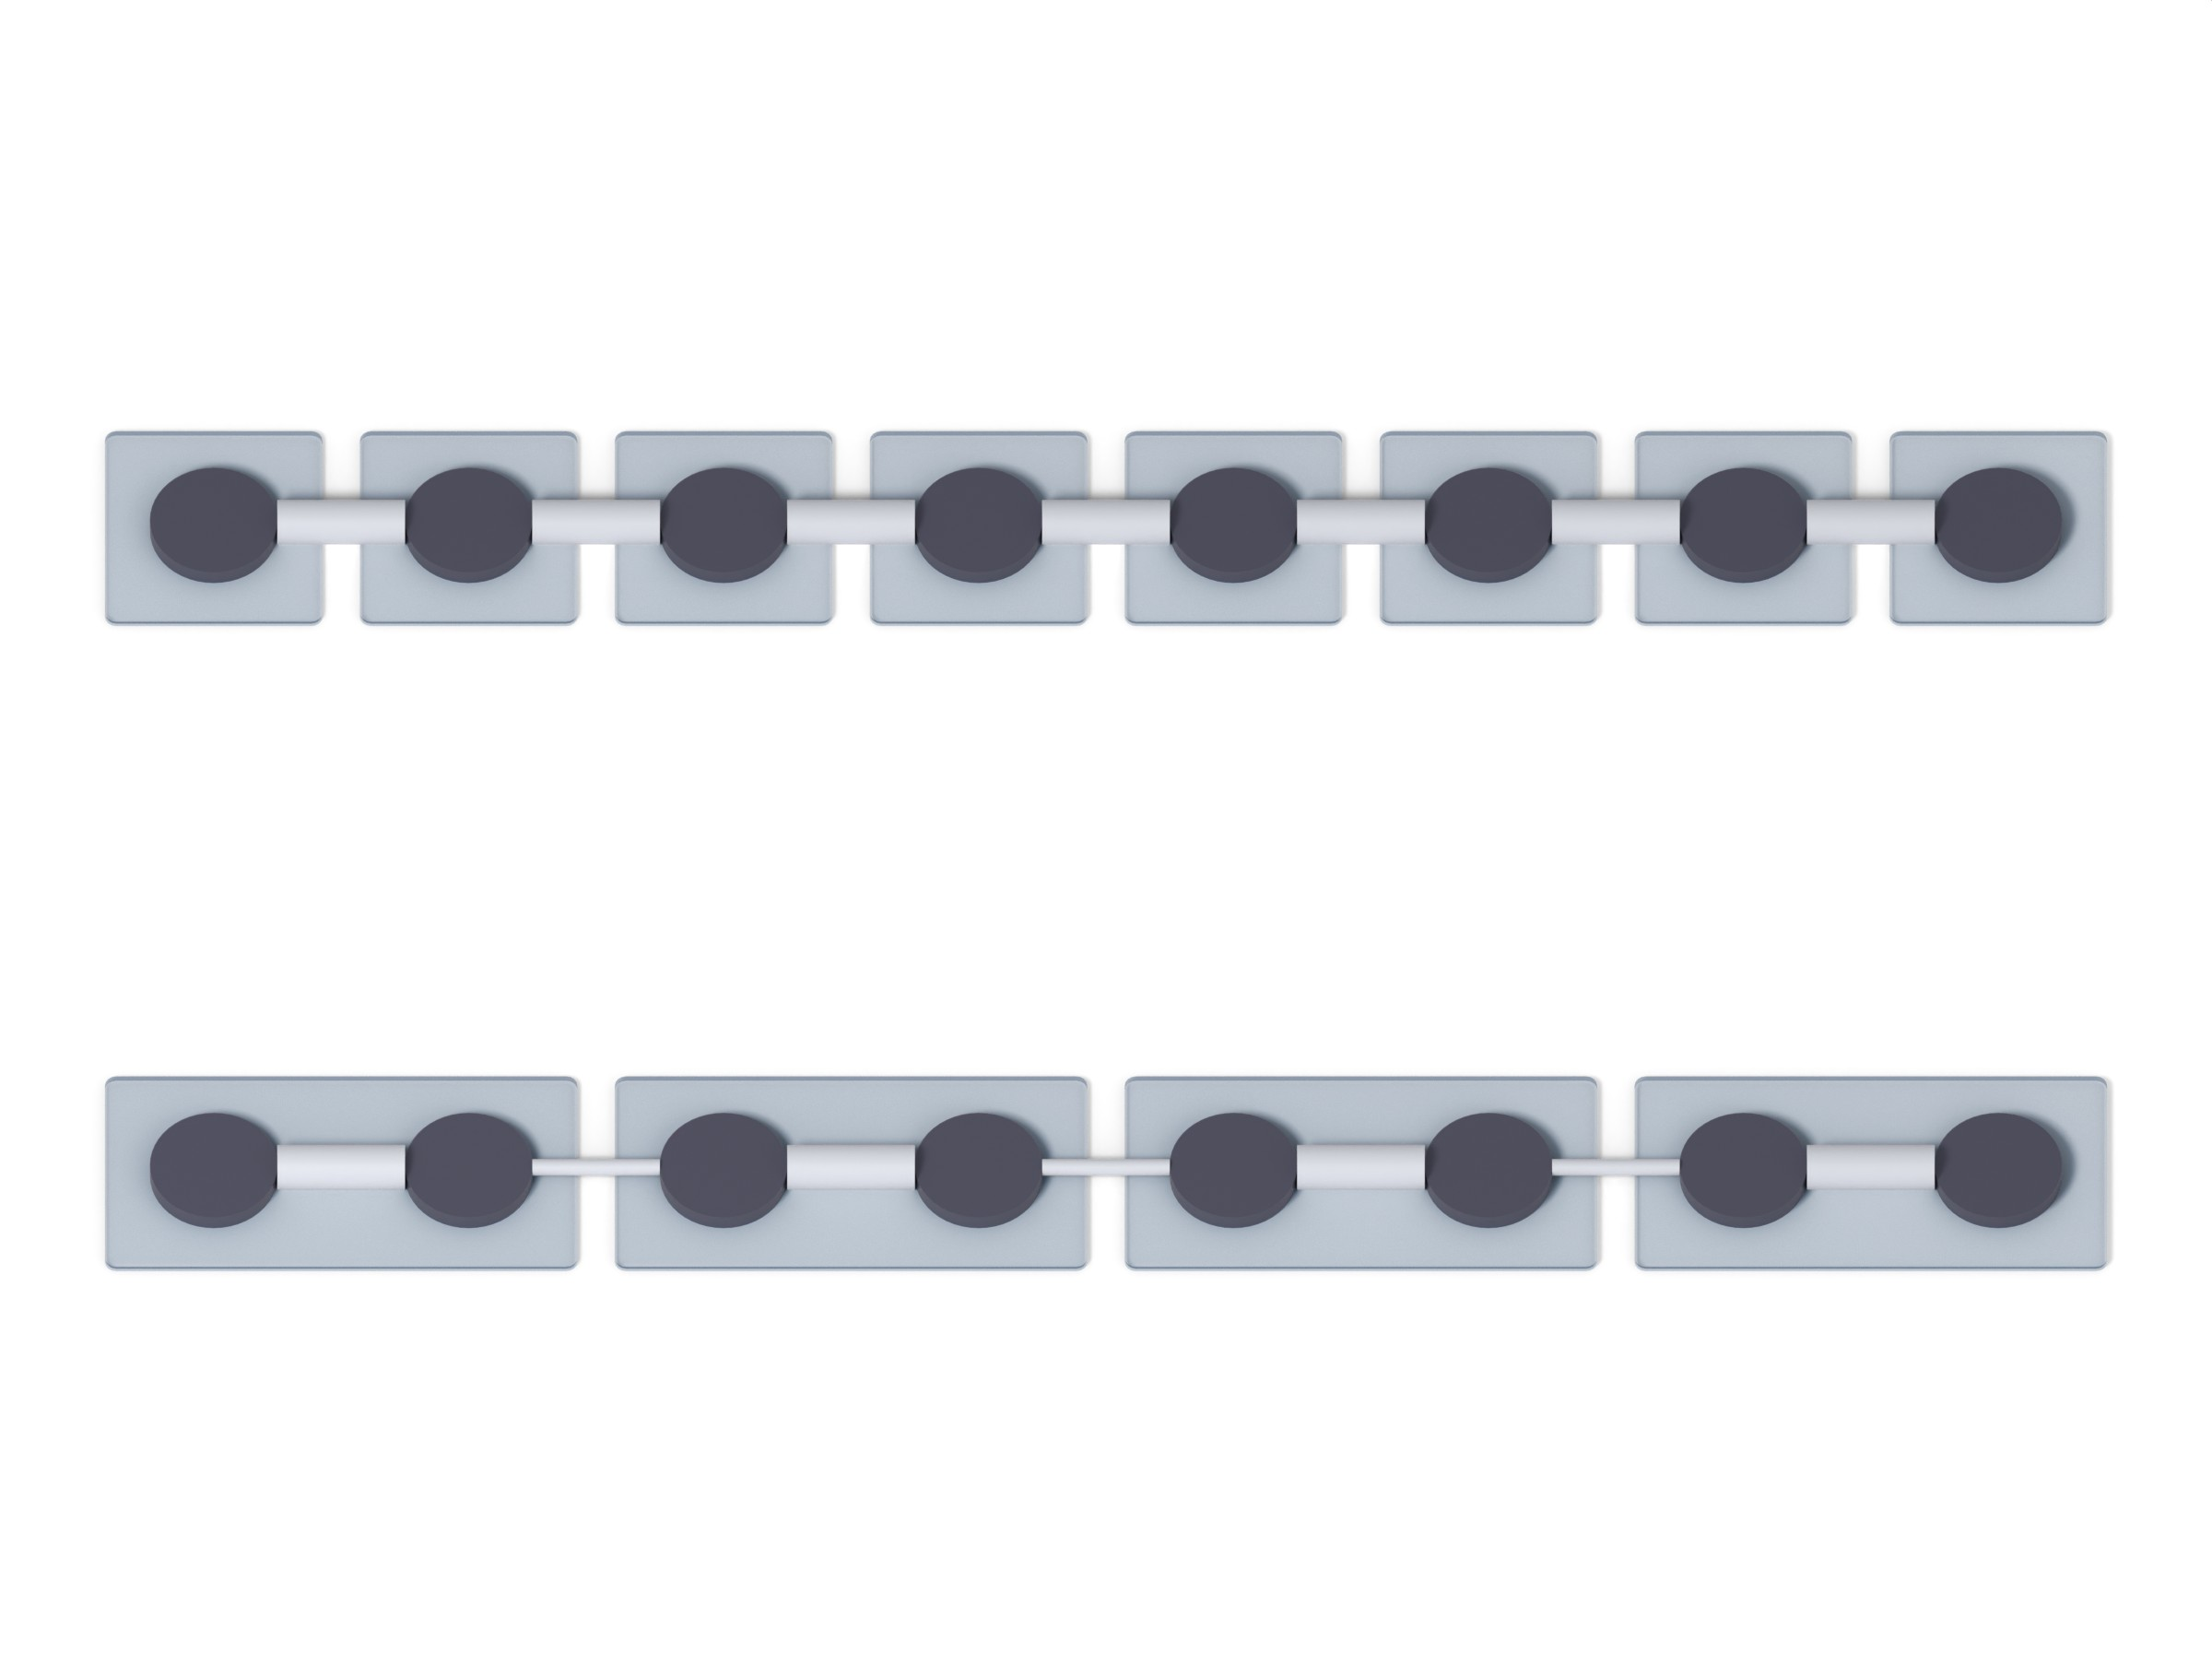
\includegraphics[width=\figw]{../blender/out/s02f03_blochrecipe_a.jpg}};
    %% written by figlib.py; x and y in units of the image width
\coordinate (aone) at (0.0458\figw,0.5759\figw);
\coordinate (atwo) at (0.0458\figw,0.2843\figw);
\coordinate (aA) at (0.7881\figw,0.2677\figw);
\coordinate (aB) at (0.9034\figw,0.2677\figw);
\coordinate (at1) at (0.8458\figw,0.1802\figw);
\coordinate (ateta) at (0.7305\figw,0.1802\figw);

    \node[lbl, anchor=south west] at (aone) {\textbf{(a)}\quad\textcolor{aqmmuted}{one site per cell}};
    \node[lbl, anchor=south west, text=aqmmuted] at (atwo) {two sites per cell};
    \node[lbl, anchor=south] at (aA) {$A$};
    \node[lbl, anchor=south] at (aB) {$B$};
    \node[lbl, anchor=north] at (at1) {$1$};
    \node[lbl, anchor=north] at (ateta) {$\eta$};
  \end{scope}
  \begin{scope}[shift={(4.6cm,0)}]
    \setlength{\figw}{11.0cm}
    \node[anchor=south west, inner sep=0pt] at (0,0)
      {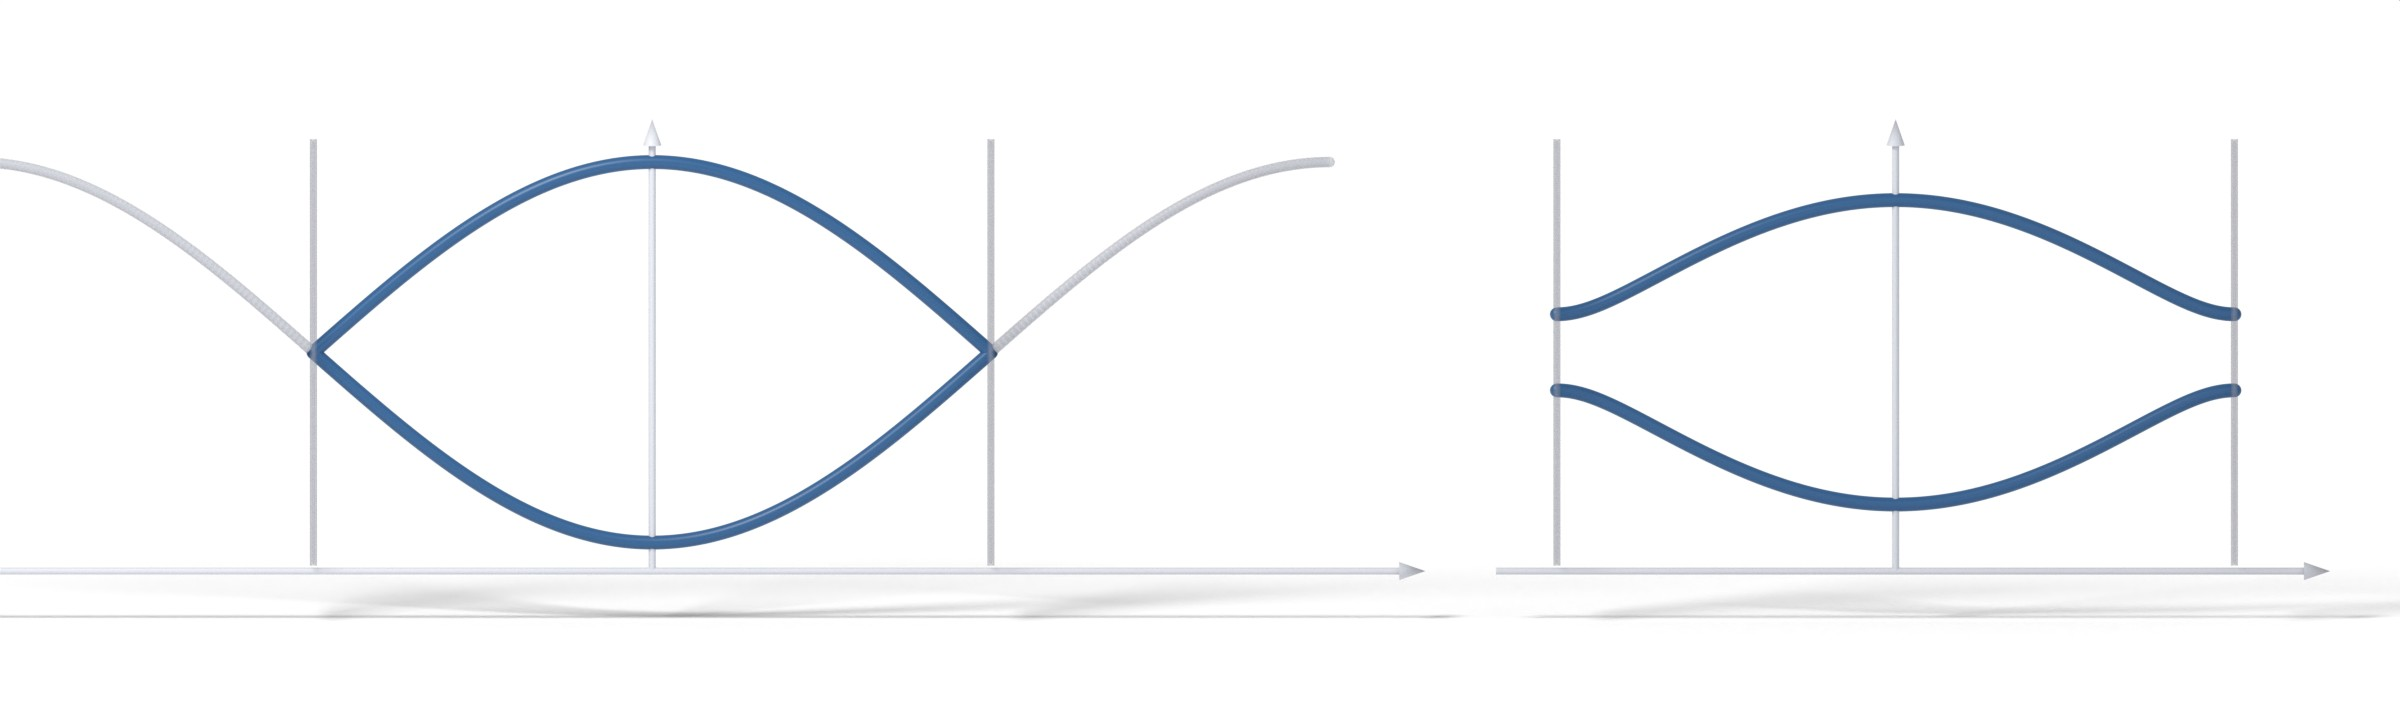
\includegraphics[width=\figw]{../blender/out/s02f03_blochrecipe_b.jpg}};
    %% written by figlib.py; x and y in units of the image width
\coordinate (bpip) at (0.4129\figw,0.0609\figw);
\coordinate (btwopip) at (0.5540\figw,0.0609\figw);
\coordinate (bpim) at (0.1306\figw,0.0609\figw);
\coordinate (btwopim) at (-0.0105\figw,0.0609\figw);
\coordinate (bphi) at (0.5939\figw,0.0629\figw);
\coordinate (bE) at (0.2717\figw,0.2511\figw);
\coordinate (bgap) at (0.4201\figw,0.1540\figw);
\coordinate (btitle) at (0.2717\figw,0.2630\figw);
\coordinate (cpip) at (0.9310\figw,0.0609\figw);
\coordinate (cpim) at (0.6487\figw,0.0609\figw);
\coordinate (cphi) at (0.9709\figw,0.0629\figw);
\coordinate (cE) at (0.7899\figw,0.2511\figw);
\coordinate (cgap) at (0.9382\figw,0.1540\figw);
\coordinate (ctitle) at (0.7899\figw,0.2630\figw);

    \node[lbl, anchor=south] at (btitle) {\textbf{(b)}\quad$\eta=1$, folded};
    \node[lbl, anchor=south] at (ctitle) {$\eta=0.6$};
    \foreach \p in {b,c} {
      \node[lbl, anchor=north] at (\p pip) {$\pi$};
      \node[lbl, anchor=north] at (\p pim) {$-\pi$};
      \node[lbl, anchor=south east] at (\p phi) {$\varphi$};
      \node[lbl, anchor=east] at (\p E) {$\epsilon$};
    }
    \node[lbl, anchor=north, text=aqmmuted] at (btwopip) {$2\pi$};
    \node[lbl, anchor=north, text=aqmmuted] at (btwopim) {$-2\pi$};
    \node[lbl, anchor=west, text=aqmbroken] at (cgap) {gap};
  \end{scope}
\end{tikzpicture}
\end{document}
